\section{Introdução}\label{sec:introducao}

% - Qual é a da coisa? (sintese c webaudio)
% - como a coisa funciona? 
%   - como um ou outro fez funcionar
%   - nosso jeito de funcionar

% -----------------------------------------------
 % http://www.charlie-roberts.com/pubs/Gibber_charles_roberts_icmc_2012.pdf


A \emph{Web Audio API} \cite{w3c_web_2012} possibilitou o processamento de sinais digitais de áudio em navegadores de rede, como por exemplo o Mozzilla Firefoz, Google Chrome ou Apple Safari \cite{roberts_web_2013,wyse_viability_2014}.  Esta API traz diversos \emph{nós de áudio} padrões, que podem ser concatenados em um grafo de DSP. Um exemplo desta concatenação é demonstrado na Figura \ref{fig:shime}.  São utilizados três instâncias de nós diferentes, em sequência, para construir um simples sintetizador. Um oscilador de ondas (OscilatorNode), ganho (\emph{GainNode}), e alto-falantes (\emph{DestinationNode}).

\begin{figure}[h]
\centering
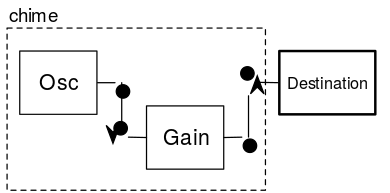
\includegraphics[scale=0.35]{chime.png}
\caption{Estrutura de síntese da API webaudio. \textbf{Fonte}: \cite{srikumar_tamming_2013}.}
\label{fig:shime}
\end{figure}

Um sintetizador mais complexo pode ter diversos nós concatenados, entre eles um nó ``especial'' chamado \emph{ScriptProcessorNode}. Uma instância deste nó permite o cálculo customizado de cada \emph{sample}. Baseado neste nó, alguns \emph{frameworks} são eles mesmos os instrumentos musicais. Por exemplo, \emph{Gibber} \footnote{disponível em \url{http://gibber.mat.ucsb.edu/})}; ou \emph{Wavepot} \footnote{Disponível em \url{http://www.wavepot.com})}\label{footnote:apps}.

Neste sentido, nossa motivação foi desenvolver um \emph{software} de luteria composicional, \emph{Termpot}, como uma experiência técnico-estética de uma pesquisa mais ampla. Esta pesquisa envolve a prática \emph{livecoding} \cite{collins_origins_2014}. O resultado não é o objetivo da pesquisa, mas envolveu uma proposta histórica de Max Mathews, \cite{mathews_groove_1970}, GROOVE, pouco discutida pela comunidade acadêmica. Esta abordagem foi fundamental para a concepção do que é \emph{livecoding}, bem como a estrutura do \emph{software} desenvolvido.

%A Seção \ref{sec:trabalhos} deste artigo apresenta os frameworks supracitados e uma breve comparação entre eles.
%A Seção \ref{sec:termpot} apresenta a ferramenta proposta.
%A Seção \ref{sec:resultados} traz os resultados desta pesquisa e a Seção \ref{sec:conclusao} apresenta as conclusões do trabalho até o presente momento.

